
\documentclass[%
 reprint,
%superscriptaddress,
%groupedaddress,
%unsortedaddress,
%runinaddress,
%frontmatterverbose, 
%preprint,
%preprintnumbers,
nofootinbib,
%nobibnotes,
%bibnotes,
 amsmath,amssymb,
 aps,
%pra,
%prb,
%rmp,
%prstab,
%prstper,
floatfix,
]{revtex4-2}
\usepackage{gensymb}
\usepackage{textcomp}
\usepackage{lipsum}
\usepackage{graphicx}% Include figure files
\usepackage{dcolumn}% Align table columns on decimal point 


\usepackage{bm}% bold math
\usepackage{siunitx}
\DeclareSIUnit\gauss{G}
\DeclareSIUnit\erg{erg}
\DeclareMathOperator{\Rot}{rot}
\sisetup{separate-uncertainty=true}
\usepackage{tabularx}
\usepackage{amssymb}
\usepackage{amsmath}
\usepackage{relsize}
\usepackage{commath}
\usepackage{enumitem}
\usepackage{xfrac}
\usepackage{float}
\usepackage{booktabs}
\usepackage{makecell}
\usepackage{caption}
\usepackage{subcaption}
\usepackage{multirow}
\usepackage[version=4]{mhchem}
\usepackage[colorlinks,bookmarks=false,citecolor=blue,linkcolor=blue,urlcolor=blue]{hyperref}
%\usepackage{hyperref}% add hypertext capabilities
%\usepackage[mathlines]{lineno}% Enable numbering of text and display math
%\linenumbers\relax % Commence numbering lines

%\usepackage[showframe,%Uncomment any one of the following lines to test 
%%scale=0.7, marginratio={1:1, 2:3}, ignoreall,% default settings
%%text={7in,10in},centering,
%%margin=1.5in,
%%total={6.5in,8.75in}, top=1.2in, left=0.9in, includefoot,
%%height=10in,a5paper,hmargin={3cm,0.8in},
%]{geometry}

\begin{document}

\preprint{APS/123-QED}

\title{Gamma-Gamma Coincidence Spectroscopy}% Force line breaks with \\


\author{Maitrey Sharma}
\email{maitrey.sharma@niser.ac.in}
\affiliation{School of Physical Sciences, National Institute of Science Education and Research, HBNI, Jatni-752050, India}




\date{\today}% It is always \today, today,
             %  but any date may be explicitly specified

\begin{abstract}
    In this experiment, we perform gamma ray spectroscopy using two detectors simultaneously and employing the use of correlation or coincidence to obtain better registration of radioactive events. We first understand the principles of nuclear physics involved, how the gammas are being produced in the radioactive source and what are the expected results in accordance with conservation of momentum and energy. The primary aim remains the verification of the same. The apparatus used is an important part of the experiment along with the software which provides the results in form of spectrum acquisition plots and summation of regions enclosed by the histograms. Finally, we discuss and draw conclusions based on the experiment, exploring its scope beyond the laboratory.
\end{abstract}

\keywords{}
\maketitle

%\tableofcontents

\section{\label{sec:level1}Introduction}
    \textbf{Gamma-ray spectroscopy} is the quantitative study of the energy spectra of gamma-ray sources. It has found immense importance in diverse fields from nuclear industry (in analysis of radioactive sources which decay by emitting gamma particles), geochemical investigations (as a surveying technique for exploration of gamma sources in soil, rocks) and astrophysics (in detection of gamma rays from distant sources emanating from the cosmos).
    \par
    Gamma rays are the highest-energy form of electromagnetic radiation, being physically the same as all other forms (e.g., X rays, visible light, infrared, radio) but having (in general) higher photon energy due to their shorter wavelength. Because of this, the energy of gamma-ray photons can be resolved individually, and a gamma-ray spectrometer can measure and display the energies of the gamma-ray photons detected.
    \par
    Most radioactive sources produce gamma rays, which are of various energies and intensities. When these emissions are detected and analyzed with a spectroscopy system, a gamma-ray energy spectrum can be produced.
    \par
    A detailed analysis of this spectrum is typically used to determine the identity and quantity of gamma emitters present in a gamma source, and is a vital tool in radiometric assay. The gamma spectrum is characteristic of the gamma-emitting nuclides contained in the source, just like in an optical spectrometer, the optical spectrum is characteristic of the material contained in a sample.
    Radioactive nuclei (radionuclides) commonly emit gamma rays in the energy range from a few $\si{\kilo \electronvolt}$ to $~\SI{10}{\mega \electronvolt}$, corresponding to the typical energy levels in nuclei with reasonably long lifetimes. Such sources typically produce gamma-ray ``line spectra'' (i.e., many photons emitted at discrete energies), whereas much higher energies (upwards of $\SI{1}{\tera \electronvolt}$) may occur in the continuum spectra observed in astrophysics and elementary particle physics. The boundary between gamma rays and X-rays is somewhat blurred, as X-rays typically refer to the high energy electronic emission of atoms, which may extend to over $\SI{100}{\kilo \electronvolt}$, whereas the lowest energy emissions of nuclei are typically termed gamma rays, even though their energies may be below $\SI{20}{\kilo \electronvolt}$.
    \begin{figure}
        \centering
        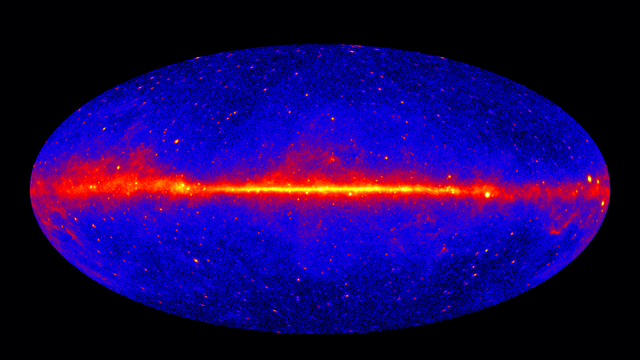
\includegraphics[scale = 0.50]{Figures/gammayrayastronomy.png}
        \caption{Survey of the sky at energies above $\SI{1}{\giga \electronvolt}$, collected by the Fermi Gamma-ray Space Telescope in five years of observation (2009 to 2013).}
        \label{fig:my_label}
    \end{figure}


\section{Description of the Set-up}
    The main components of a gamma spectrometer are the energy-sensitive radiation detector and the electronic devices that analyse the detector output signals, such as a pulse sorter (i.e., multichannel analyzer or MCA). Other important components include the signal processing electronics (pre-amplifier, shaping amplifier) and a power supply.
    \subsection{The Detector}
    Gamma spectroscopy detectors are passive materials that are able to interact with incoming gamma rays. The most important interaction mechanisms are the photoelectric effect, the Compton effect, and pair production. Through these processes, the energy of the gamma ray is absorbed and converted into a voltage signal by detecting the energy difference before and after the interaction (or, in a scintillation counter, the emitted photons using a photomultiplier).
    \par
    Scintillation detectors use crystals that emit light when gamma rays interact with the atoms in the crystals. The intensity of the light produced is usually proportional to the energy deposited in the crystal by the gamma ray. This experiment consists of scintillation detector in which a $\SI{10}{\milli \metre} \times \SI{10}{\milli \metre} \times \SI{8}{\milli \metre}$ scintillator is mated to a semiconductor $p-n$ junction connected in reverse bias mode. The depletion region thus created acts as an ionisation medium which converts the scintillation photons into a corresponding number of electron-hole pairs. The small amount of charge generated as a result of one gamma ray depositing its entire energy in the scintillator which then gets converted into a charge pulse by the $p-n$ junction results in an event in the photopeak region. Other types of interactions such as Compton scattering result on different energies being detected. This charge pulse is then fed to the signal processing electronics, followed by the multi-channel analyzer (MCA) which generates a spectrum.
    \par
    The detector used in this instrument has $\SI{10}{\milli \metre} \times \SI{10}{\milli \metre}$ surface area with an entry window of $\SI{8}{\milli \metre}$ diameter. The window is covered with a thin aluminium foil to keep out visible light.
    \subsection{Signal processing electronics}
    The charge generated by an incident bunch of scintillation photons is converted into a corresponding output voltage by utilising a charge sensitive preamplifier. The main role of the preamp is to ensure impedance matching between high impedance at the detector side (i.e. input), with the low output impedance of the post-processing electronics. This also improves the signal-to-noise ratio (SNR).
    \par
    The output of the Shaping amplifier is a Guassian shaped pulse. The amplitude varies from 0 to $\SI{3.3}{\volt}$, depending on the deposited energy. The shaping amplifier’s gaussian pulse output goes to the input of the built-in MCA.
    \subsection{Multi-channel Analyzer}
    The hardware performs a variety of tasks ranging from detection of the pulse, post-processing of the signal, and sorting the signals on the basis of their peak height into predefined bins. The MCA does the sorting and histogram generation, and it is designed to have 1024 channel (1K) resolution, with an input voltage range of $0-\SI{3.3}{\volt}$.
    \par
    Input pulses are only accepted if the amplitude exceeds a threshold value (to reject low energy peaks which might not be due to gamma rays) which is set to 75 channels.
    \begin{figure}
        \centering
        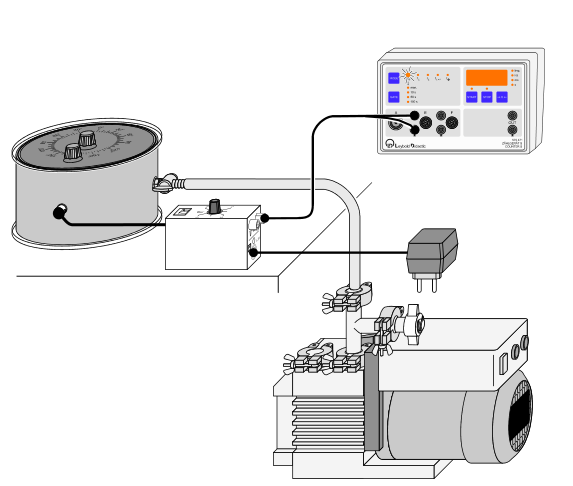
\includegraphics[scale = 0.33]{Figures/setup.png}
        \caption{A labelled graphic of the equipment. The radioactive source is kept in front of the gamma detector window, and has been removed while taking the photo to show the window.}
        \label{fig:setup}
    \end{figure}
    
    
\section{Theory}
    $^{22}Na$ radioactively decays to an excited state of $^{22}Ne$ either by emission of a positron (90\%probability) or by electron capture (10\% probability). The excited $^{22}Ne$ nucleus decays with a mean life $\SI{3e-12}{\second}$ to the ground state with the emission of a $\SI{1.274}{\mega \electronvolt}$ gamma.
    \begin{figure}
        \centering
        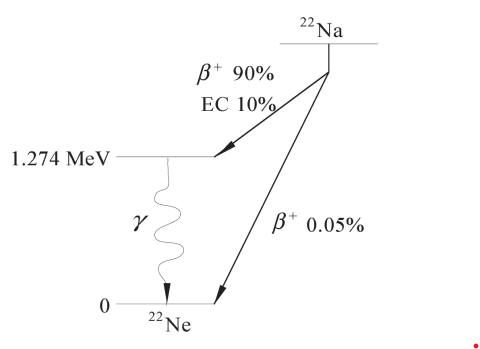
\includegraphics[scale = 0.8]{Figures/na-22.png}
        \caption{The decay of $^{22}Na$ proceeds by positron $\beta^+$ emission (90\%) or electron capture (10\%) to produce an excited state of $^{22}Ne$ which decays by emission of a $\SI{1.274}{\mega \electronvolt}$ gamma.}
        \label{fig:my_label}
    \end{figure}
    \par
    The positrons are emitted with a range of kinetic energies up to about $\SI{0.5}{\mega \electronvolt}$. They lose this energy quickly ($\SI{e-9}{\second}$) in the material surrounding the source and, when they reach atomic ($\si{\electronvolt}$) energies, capture an electron to form positronium—a hydrogen-like ``atom''. The positronium decays (with a lifetime on the order of $\SI{e-10}{\second}$) by annihilation of the $e^+$ and $e^-$ into two gammas. By energy conservation, the energy of the gammas must equal the energy (including the rest mass energy) of the positronium and, by momentum conservation, the net momentum of the two gammas must equal the initial momentum of the positronium. 
    \par
    The magnitude of the photon momentum is given by
    \begin{equation}
        p_{\gamma} = \dfrac{E_{\gamma}}{c}
    \end{equation}
    In the rest frame of the positronium, there is no initial momentum and thus the two annihilation gammas must be of opposite momentum in that frame. Consequently, the two photons must be equal in energy and propagate in opposite directions. Since the initial energy of the positronium (neglecting the binding energy of a few $\si{\electronvolt}$) is simply the rest mass energy of an electron and positron ($\SI{511}{\kilo \electronvolt}$ each), each gamma will have an energy $E_{\gamma} = \SI{511}{\kilo \electronvolt}$.
    \par
    In the laboratory frame, the positronium will be moving with a range of kinetic energies up to a few eV (typical energy of electrons with which it forms). Then, depending on the direction of the initial positronium momentum relative to the gamma emission direction, the transformation to the lab frame gives gamma energies that might differ from $\SI{511}{\kilo \electronvolt}$ and/or produce gammas that are not emitted exactly $180 \degree$ apart.
    \par
    There are three dominant gamma-ray interactions with matter: the photoelectric effect, the Compton effect and pair production.
    \par
    The photoelectric effect is a common interaction between a low-energy gamma ray and a material. In this process the photon interacts with an electron in the material losing all of its energy. The electron is ejected with an energy equal to the initial photon energy minus the binding energy of the electron. This is a useful process for spectroscopy since an output pulse in a detector is produced that is proportional to the gamma-ray energy, as all of the energy of the gamma ray is transferred to the detector. This produces a characteristic full-energy peak in the spectrum that can be used for the purpose of identifying the radioactive material.
    \par
    The photon can scatter by a free electron and transfer an amount of energy that depends on the scattering angle. This process is called Compton scattering. The energy of the scattered photon $E'$ is
    \begin{equation}
        E' = \dfrac{E}{1 + \dfrac{E}{m_0 c^2} (1 \cos \theta)}
    \end{equation}
    where $E$ is the incident gamma-ray energy and $\theta$ is the angle of scatter. The term $m_0 c^2$ is the rest mass of the electron, equal to $\SI{511}{\kilo \electronvolt}$. The energy given to the electron is
    \begin{equation}
        E_e = E - E'
    \end{equation}
    The maximum energy given to an electron in Compton scattering occurs for a scattering angle of $180 \degree$, and the energy distribution is continuous up to that point (since all scattering angles up to $180 \degree$ are possible). This energy, known as the Compton edge, can be calculated from the incident gamma ray energy.
    \par
    For $\theta = 180 \degree$,
    \begin{equation}
        E' = \dfrac{E}{1 + \dfrac{2E}{m_0 c^2}}
    \end{equation}
    The actual energy deposited depends upon the angle of scatter as described in the equations above. The spectrum shows that many pulses have energies in a range below the Compton edge – called the Compton Continuum.
    \par
    Pair production can occur when the gamma-ray energy is greater than $\SI{1.022}{\mega \electronvolt}$ and is a significant process at energies above $\SI{2.5}{\mega \electronvolt}$. The process produces a positron and electron pair that slow down through scattering interactions in the material. When the positron comes to rest, it annihilates with an electron producing a pair of $\SI{511}{\kilo \electronvolt}$ gamma rays that are produced back-to-back. These can be absorbed through the photoelectric effect to produce full-energy peaks at $\SI{511}{\kilo \electronvolt}$. A component due to Compton scattering can also be observed. When a photon interacts with the crystal through pair production, one or both of the annihilation photons can escape undetected from the crystal. If one of the photons escapes undetected, then this will result in a peak in the spectrum at an energy of $\SI{511}{\kilo \electronvolt}$ less than the full-energy peak. This is called the single escape peak. Similarly, if both photons escape undetected, a peak will appear $\SI{1.022}{\mega \electronvolt}$ below the full-energy peak, called the double escape peak.
    \par
    As the radioactive source decays, the two detectors placed facing each other, detect the incident gammas. The term ``coincidence'' here corresponds to a detection of a gamma of same energy and at the same time by both the detectors. Coincidence measurements using multiple spectrometers allows for better identification of events with simultaneous multiple gamma emissions.
    \begin{figure}
        \centering
        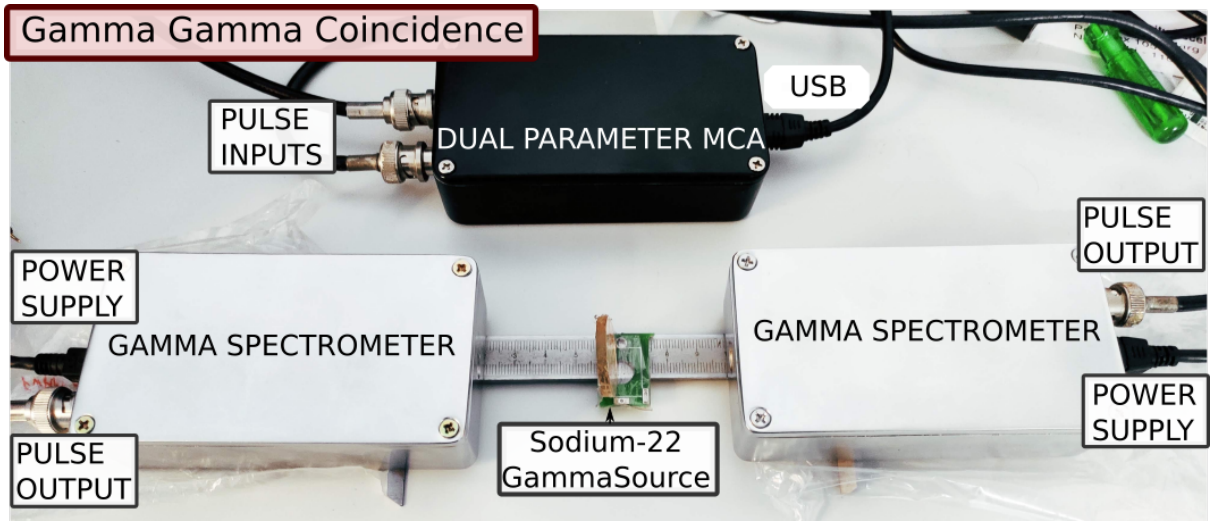
\includegraphics[scale = 0.33]{Figures/setup2.png}
        \caption{Two gamma spectrometers placed with a $^{22} Na$ positron source in the middle. The dual MCA carries out the data acquisition.}
        \label{fig:my_label}
    \end{figure}
    
    
\section{Calibration}
    Before taking the observations, it is essential to calibrate the set-up using the MCA. Our radioactive source $^{22} Na$ has has a photopeak at $\SI{511}{\kilo \electronvolt}$ from positron annihilation, and a high energy peak at 1275. We will use the $\SI{511}{\kilo \electronvolt}$ peak for calibrating the dual MCA. Calibration is done as follows:
    \begin{enumerate}
        \item The source is placed in front of the detector window, and the corresponding spectrum is acquired over a period of 90 minutes.
        \item After spectrum acquisition, the first input trace is selected, followed by insertion of a selection region around the $\SI{511}{\kilo \electronvolt}$ photopeak, ensuring it is well-covered.
        \item This selected part is now fitted by entering the known energy of the peak against the channel number extracted from the peak and calibration is applied.
        \item The same process is repeated for the second input trace (from the second detector) and finally, the calibration process is complete.
    \end{enumerate}
\section{Observations}
    The software used to record the spectrum acquisition plot is CNSPEC by CSpark Research.
    \par
    The spectrum acquisition plot when the source was placed in the middle of the two detectors at $180 \degree$ of each other is given in figure (\ref{fig:180spec}) and after isolation of counts by application of energy gates is given in (\ref{fig:180gate}). The 3-D heat map thus obtained is given in figure (\ref{fig:3d}) and the corresponding 2-D heat map is given in (\ref{fig:2d}). 
    \par
    Similarly, the spectrum acquisition plots for when the detectors are perpendicular to each other is given in (\ref{fig:90spec}) and after isolation of counts by application of energy gates is given in (\ref{fig:90gate}). The corresponding figures for 2 more positions around $180 \degree$ (viz. $184 \degree$ and $176 \degree$) are given in figures (\ref{fig:184spec}), (\ref{fig:184gate}), (\ref{fig:176spec}) and (\ref{fig:176gate}) respectively.
    \begin{figure}
        \centering
        \begin{subfigure}[b]{0.5\textwidth}
            \centering
            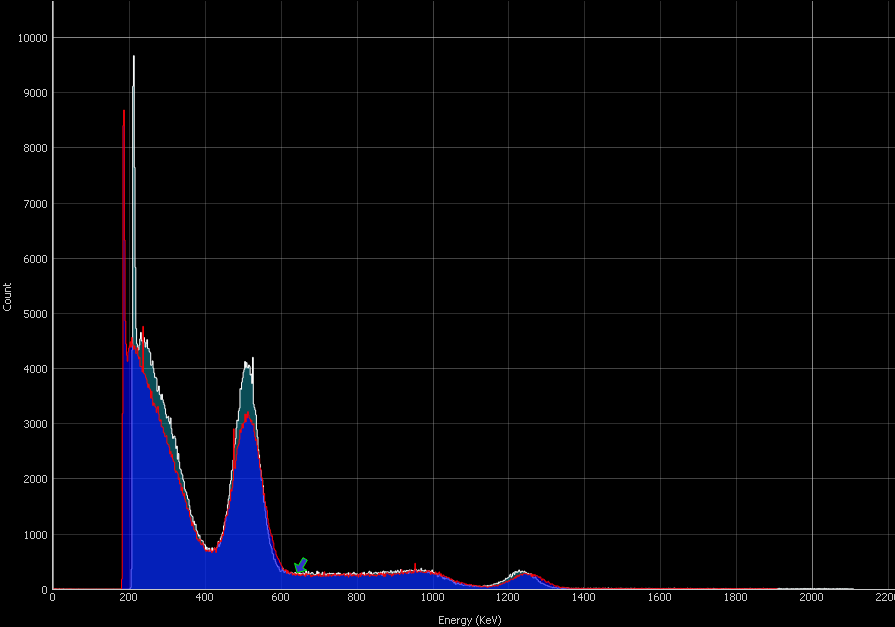
\includegraphics[scale = 0.35]{Figures/spectrum_acquisition_180.png}
            \caption{Before the application of gates}
            \label{fig:180spec}
        \end{subfigure}
        \hfill
        \begin{subfigure}[b]{0.5\textwidth}
            \centering
            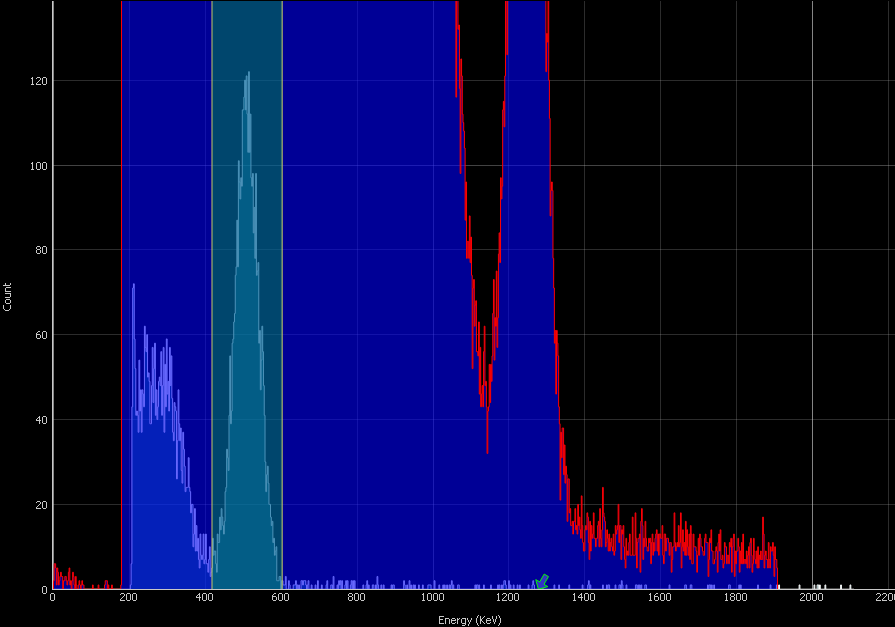
\includegraphics[scale = 0.35]{Figures/after_gate_180.png}
            \caption{After the application of gates}
            \label{fig:180gate}
        \end{subfigure}
            \caption{Spectrum acquisition plots when the detectors are place at an angle of $180 \degree$ with one another}
            \label{fig:180}
    \end{figure}
    \begin{figure}
        \centering
        \begin{subfigure}[b]{0.5\textwidth}
            \centering
            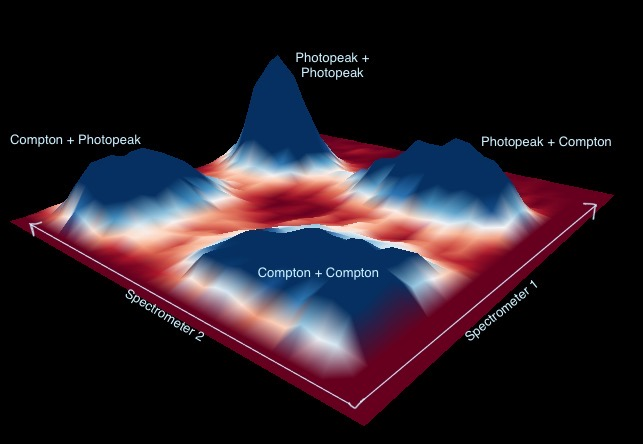
\includegraphics[scale = 0.35]{Figures/3D_heat_map.jpg}
            \caption{3-D heat map}
            \label{fig:3d}
        \end{subfigure}
        \hfill
        \begin{subfigure}[b]{0.5\textwidth}
            \centering
            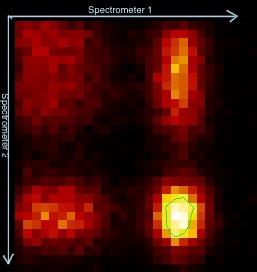
\includegraphics[scale = 0.8]{Figures/2D_heat_map.jpg}
            \caption{2-D heat map}
            \label{fig:2d}
        \end{subfigure}
            \caption{Heat maps corresponsing to the plot when the detectors are place at an angle of $180 \degree$ with one another}
            \label{fig:heat}
    \end{figure}
    \begin{figure}
        \centering
        \begin{subfigure}[b]{0.5\textwidth}
            \centering
            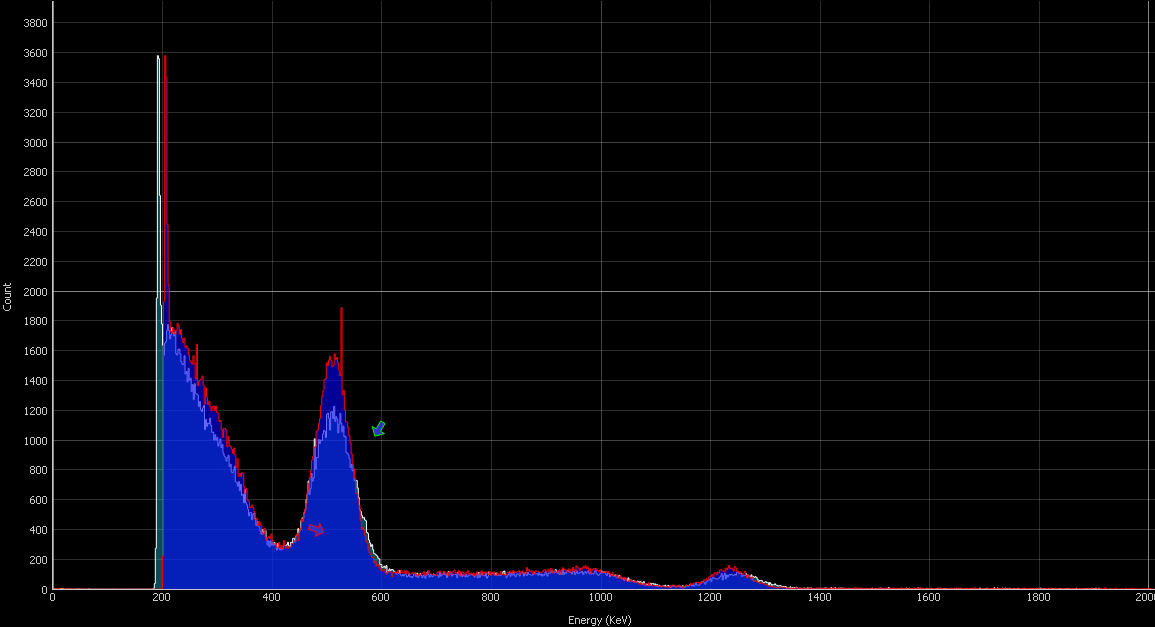
\includegraphics[scale = 0.27]{Figures/spectrum_acquisition_90.png}
            \caption{Before the application of gates}
            \label{fig:90spec}
        \end{subfigure}
        \hfill
        \begin{subfigure}[b]{0.5\textwidth}
            \centering
            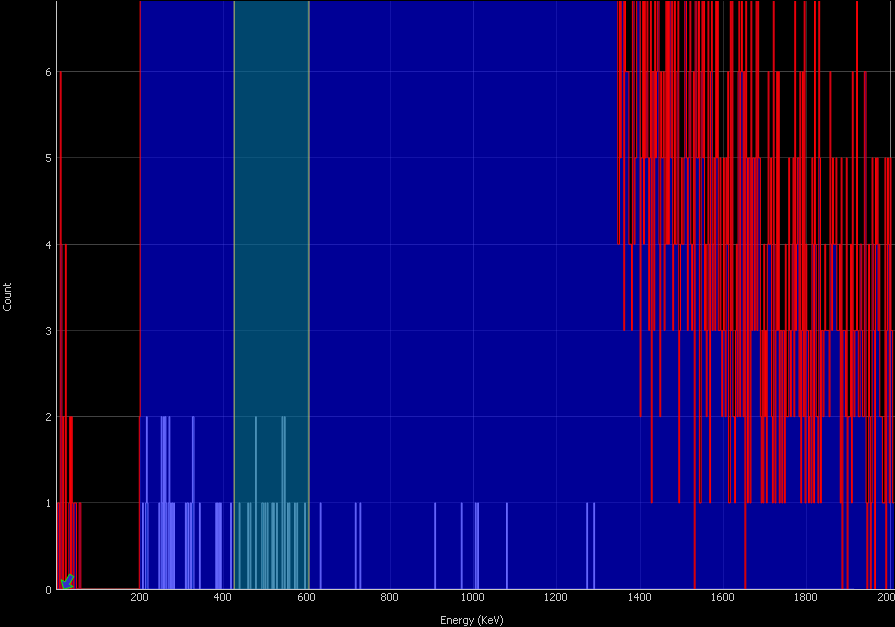
\includegraphics[scale = 0.35]{Figures/after_gate_90.png}
            \caption{After the application of gates}
            \label{fig:90gate}
        \end{subfigure}
            \caption{Spectrum acquisition plots when the detectors are place at an angle of $90 \degree$ with one another}
            \label{fig:90}
    \end{figure}
    \begin{figure}
        \centering
        \begin{subfigure}[b]{0.5\textwidth}
            \centering
            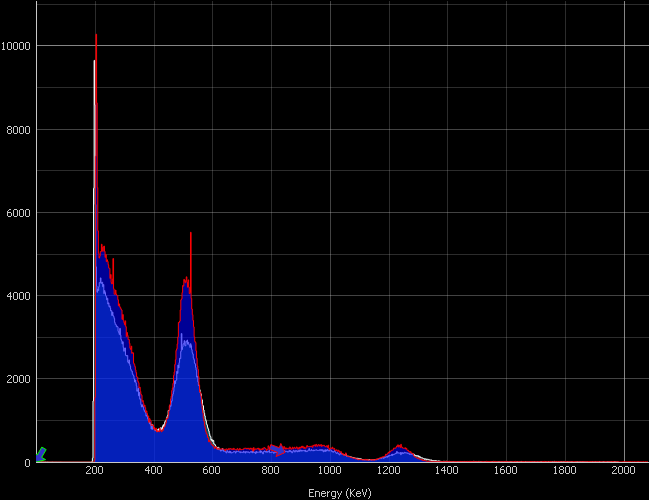
\includegraphics[scale = 0.50]{Figures/spectrum_acquisition_184.png}
            \caption{Before the application of gates}
            \label{fig:184spec}
        \end{subfigure}
        \hfill
        \begin{subfigure}[b]{0.5\textwidth}
            \centering
            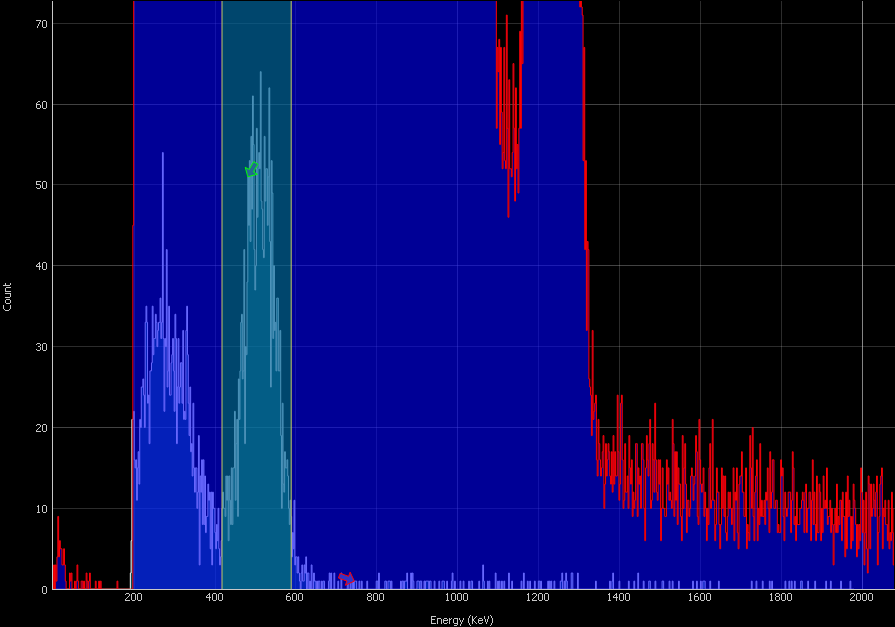
\includegraphics[scale = 0.35]{Figures/after_gate_184.png}
            \caption{After the application of gates}
            \label{fig:184gate}
        \end{subfigure}
            \caption{Spectrum acquisition plots when the detectors are place at an angle of $184 \degree$ with one another}
            \label{fig:184}
    \end{figure}
    \begin{figure}
        \centering
        \begin{subfigure}[b]{0.5\textwidth}
            \centering
            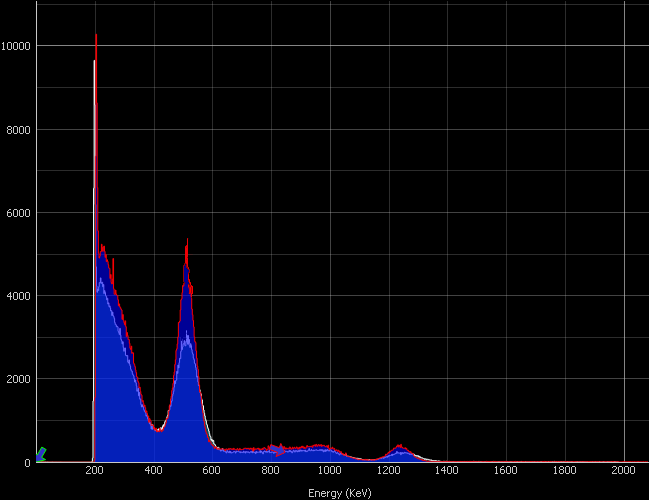
\includegraphics[scale = 0.55]{Figures/spectrum_acquisition_176.png}
            \caption{Before the application of gates}
            \label{fig:176spec}
        \end{subfigure}
        \hfill
        \begin{subfigure}[b]{0.5\textwidth}
            \centering
            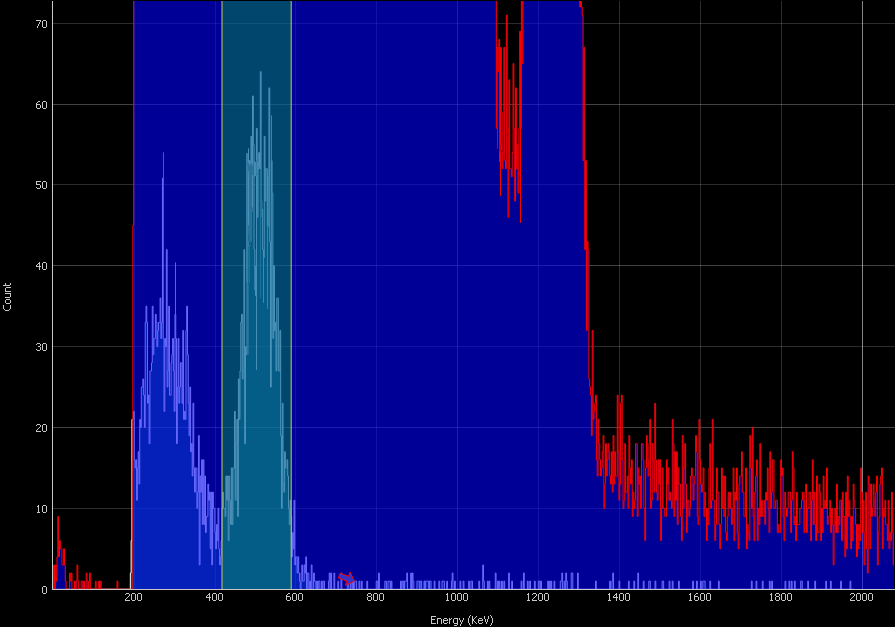
\includegraphics[scale = 0.45]{Figures/after_gate_176.png}
            \caption{After the application of gates}
            \label{fig:176gate}
        \end{subfigure}
            \caption{Spectrum acquisition plots when the detectors are place at an angle of $176 \degree$ with one another}
            \label{fig:176}
    \end{figure}

    
\section{Discussions}
    \begin{enumerate}
        \item The number of coincident counts after application of gates for when the detectors were at $180 \degree$ was obtained as 4258.
        \item The number of coincident counts after application of gates for when the detectors were at $90 \degree$ was obtained as 21.
        \item The number of coincident counts after application of gates for when the detectors were at $184 \degree$ was obtained as 2687.
        \item The number of coincident counts after application of gates for when the detectors were at $176 \degree$ was obtained as 3143.
        \item We observe that maximum coincidences are obtained when detectors are placed at an angle of $180 \degree$ to each other. This is expected as from the conservation of momentum and energy. The same energy gammas, when created, are emitted in opposite directions.
        \item The number of coincidences obtained at $90 \degree$ is very less, as expected as there would be very few, if any, gammas that would be deviating that much and violating the conservation of momentum. This small number might as well considered well within the margin of error and ideally the number of coincidences should have been equal to zero.
        \item The number of coincidences obtained at $184 \degree$ and $176 \degree$ are marginally less that what obtained at $180 \degree$ but still substantial.
        \item In the lab frame the two annihilation gammas are emitted within few degrees or less of $180 \degree$ from one another. This is expected behavior.
        \item This can be explained by imagining a \textit{flux of possible coincidence gammas} moving in the opposite direction.
        \item This flux (let us call it $c$-flux is not the same as the raw flux of $\SI{511}{\kilo \electronvolt}$ gammas from the source. It is not uniform; it extends only into the region opposite the fixed detector from the source. With both detectors at the same distance $R$ from the source, the $c$-flux will be the product of the raw flux at that distance and the probability that the fixed detector will register a count in the photopeak. In the region opposite the aperture, it is reduced in intensity from the raw flux by the photopeak efficiency.
        \item The $c$-flux is a real flux of gammas radiating out from the source opposite the fixed detector. It is modeled based on the assumption that the $\SI{511}{\kilo \electronvolt}$ gammas are always created in $180 \degree$ pairs. The $c$-flux is simply a selected fraction of the total flux, for which the opposite gamma of the pair is detected in the fixed detector. Consequently, any of the $c$-flux gammas detected in the movable detector's photopeak will be counted as coincidences.
        \item Real coincidences should only occur when there is some overlap of the movable detector into the region of the $c$-flux. If the fixed and movable detectors are very far from being opposite one another, there will be no overlap and no chance of real coincidences.
        \item There is a finite probability that of the two signals being registered, one will arrive in each detector near enough in time to be counted as a coincidence. The average rate at which these random coincidences can be expected to occur is easily calculated and depends on the singles rates and the width $\tau$ of the gating signal.
        \item There are various direct applications of this experiment. We can study the decay patterns of various radioactive elements. It is also possible to study the energy loss of gamma rays in materials, by using attenuators. One can also carry out dosimetry applications, or $\dfrac{1}{r^2}$ dependence of counts.
        \item We can analyze energy spectrum of gamma sources such as $^{137} Cs$. Cesium 137 is a radioactive isotope that emits gamma rays at $\SI{662}{\kilo \electronvolt}$. Its monoenergetic nature makes it ideal for single point calibration.
        \item The sandy beaches in southern India are rich in Thorium-232, as well as natural uranium. The activity is low, and of the order for a few ten counts per second for a gram of monazite sand, so spectrum must be acquired for a few hours to get good data. Energies such as $\SI{2.6}{\mega \electronvolt}$ from Thallium-208 can be clearly identified. The double escape peak from the same source can also be spotted around $\SI{1.6}{\mega \electronvolt}$.
        \item In nuclear physics applications, coincidence systems are used to detect and identify weak detection signals or to distinguish a physics signal from background signals, as is done in Compton suppression or cosmic veto systems.
        \item In high-energy or particle physics, detection systems consisting of thousands of detectors and electronics channels are all operated in coincidence when two accelerated beams collide to search for newly formed particles or new decay pathways.
    \end{enumerate}

\section{Precautions}
    \begin{enumerate}
        \item The radioactive sources should be held with utmost care.
        \item The energy calibration should be performed before taking the readings, for which it is essential to make a .csv files beforehand which in which the data will be saved (continuously).
    \end{enumerate}
\section{Conclusions}
    The results obtained through the experiment were satisfactory and as expected.






\end{document}
%
% ****** End of file apssamp.tex ******
